\documentclass{beamer}

\usepackage[utf8]{inputenc}
\usepackage[frenchb]{babel}
\usepackage{lmodern}
\usepackage{amsmath}
\usepackage{graphicx}
\usepackage{amssymb}
\usepackage{numprint}
\usepackage[squaren,Gray]{SIunits}
\usepackage{tikz}
\usepackage{pgfplots}
\usepackage{mathrsfs}
\usetheme{Warsaw}

\title{APP3: Le rayonnement électromagnétique}
\author{Groupe 1254}
%\author{\bsc{Paulus} L.,\bsc{Joachim} C. , \bsc{Goyens} V., \bsc{Boigelot} S., \bsc{Xavier} L., \bsc{Sliti} A., \bsc{Nicol} E.}

\begin{document}
\begin{frame}
	\maketitle
\end{frame}
\begin{frame}{Question 1}
	\begin{columns}
		\begin{column}{0.40\textwidth}
			\begin{center}
	    		\includegraphics[scale=0.3, angle=90]{question1.png}
        		\end{center}
		\end{column}
		\begin{column}{0.40\textwidth}
		Le circuit forme une capacité.
		Les lois de Kirchhoff sont bien respectées : il y a un courant entre les deux fils colinéaires. Il s'agit 			d'un \emph{courant de déplacement}.
		\end{column}
	\end{columns}
\end{frame}
\begin{frame}{Question 1: un seul fil}
%
%        	\end{column}
%        	\begin{column}{0.40\textwidth}
%			\begin{center}
%	    Différence de tension entre les deux extrémités $\Rightarrow$ capacité.
%	    \\Les lois de Kirchhoff ne sont pas perturbées.
%        	\end{center}
%        	\end{column}
%        	\end{columns}
%        	
%        	\end{frame}
%\begin{frame}{Question 1}
%version d'Edward
	\begin{columns}
		\begin{column}{0.40\textwidth}
			\begin{center}
	    		\includegraphics[scale=0.2, angle=90]{Question1-2.png}
        		\end{center}
        	\end{column}
%<<<<<<< HEAD
%		\begin{column}{0.40\textwidth}
%		De nouveau, les lois de Kirchhoff sont respectées, ici de manière évidente.
%		\end{column}
%	\end{columns}
%======= version de Xavier
        	\begin{column}{0.40\textwidth}
			\begin{center}
	    Pour un seul fil: le système est fermé.
	    
	    Pas de problème avec les lois de Kirchhoff 
        	\end{center}
        	\end{column}
        	\end{columns}
\end{frame}
\begin{frame}{Question 2}
	\begin{columns}
		\begin{column}{0.60\textwidth}
			\begin{center}
	    		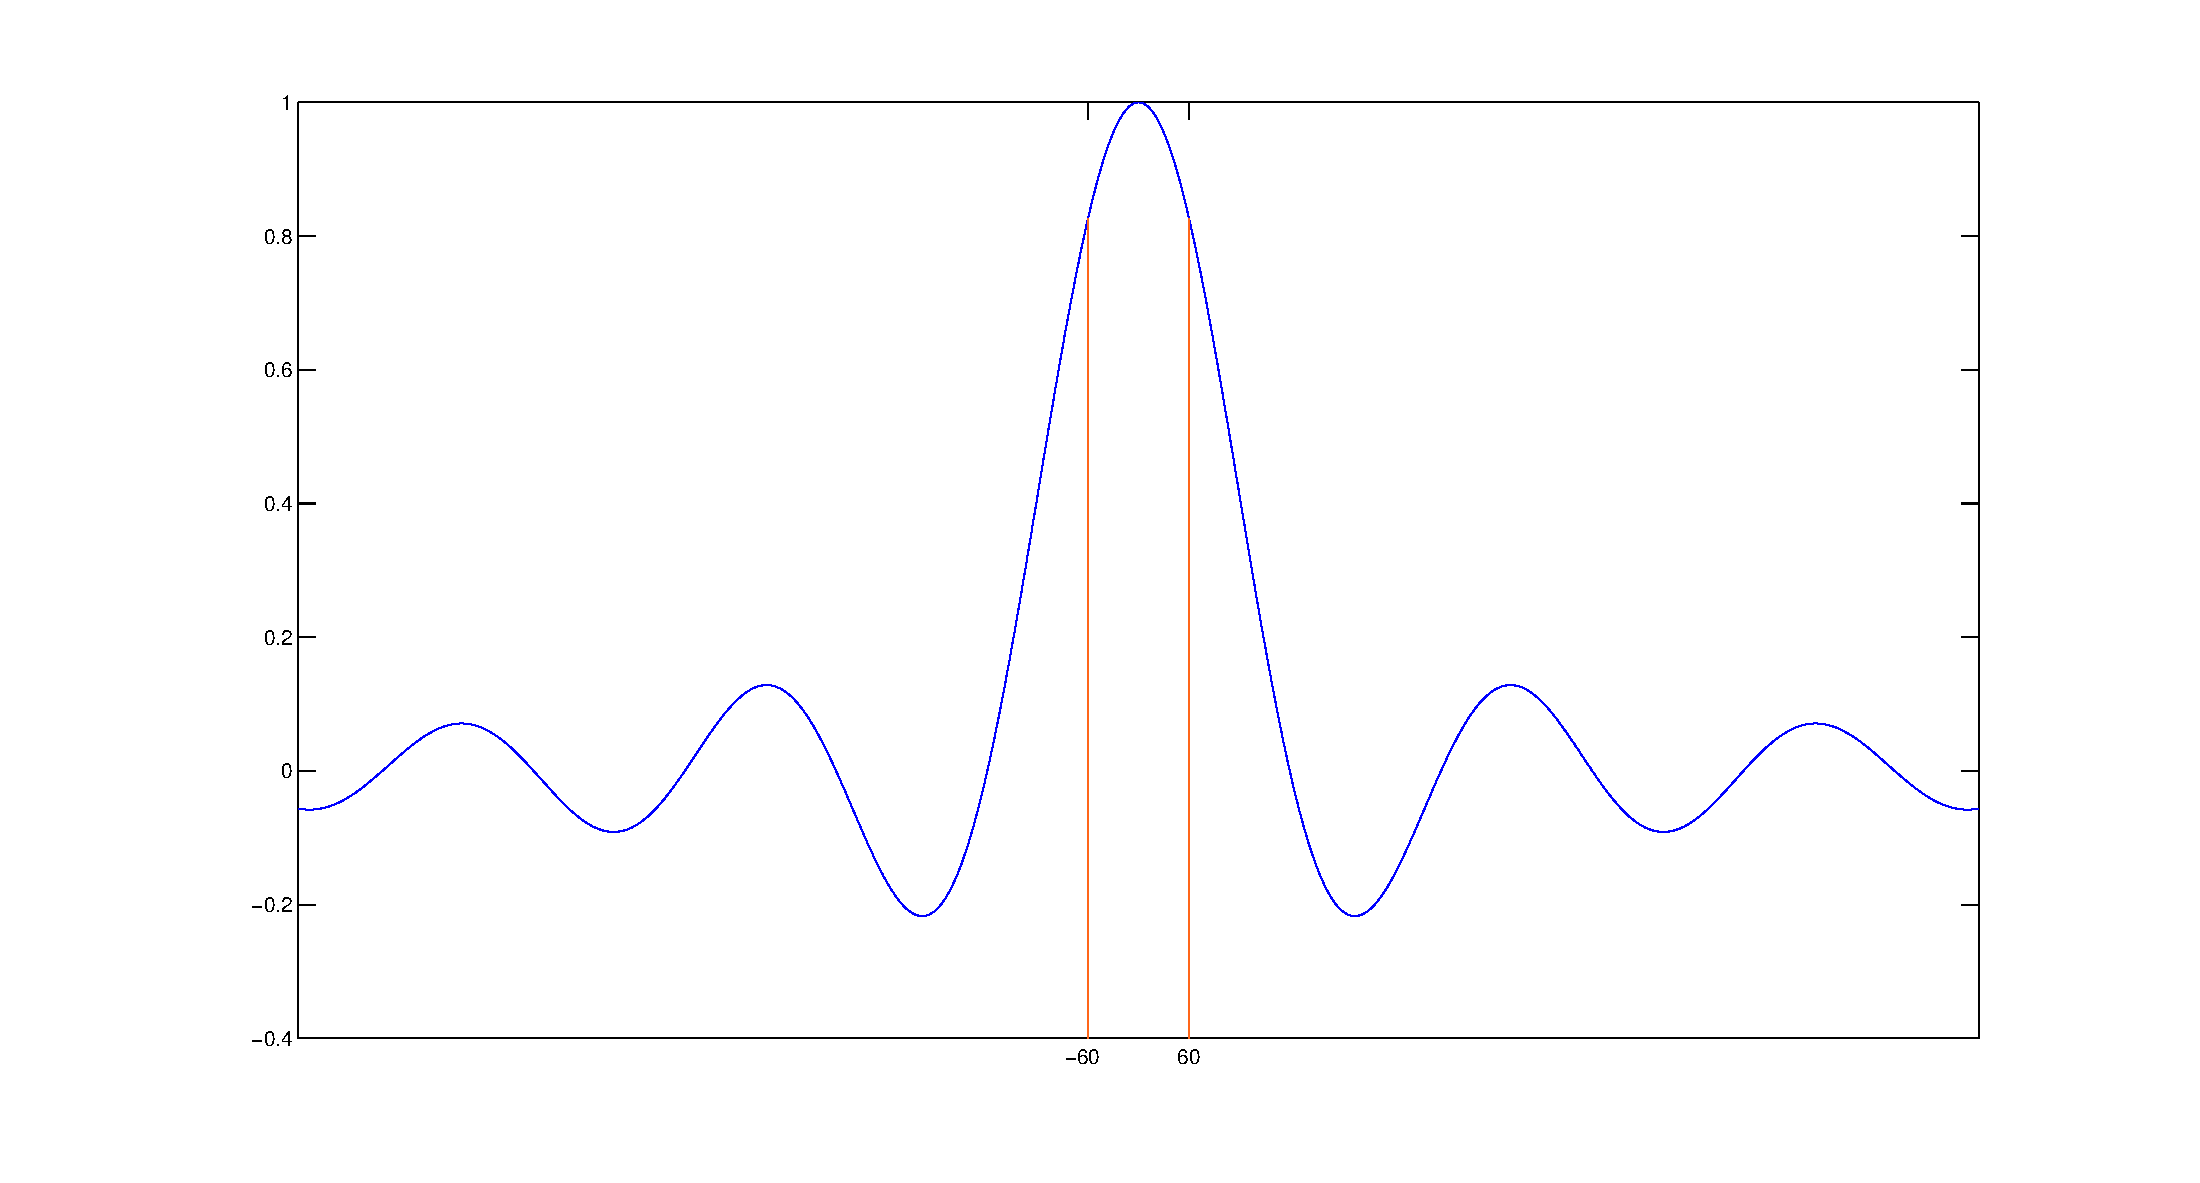
\includegraphics[scale=0.21]{sinxx.eps}
        		\end{center}
        	\end{column}
        	\begin{column}{0.35\textwidth}
			\begin{center}
	    \begin{enumerate}
	    \item 1 antenne:$$ \left( \frac{\sin x}{x}\right)^2$$
	    \item $n$ antennes: $$ \left( \frac{\sin nx}{\sin x}\right)^2 \cdot \left( \frac{\sin x}{x}\right)$$
	    \end{enumerate}
	    
        	\end{center}
        	\end{column}
        	\end{columns}
\end{frame}
\begin{frame}{Question 2}
	\begin{columns}
		\begin{column}{0.40\textwidth}
			\begin{center}
	    		\includegraphics[scale=0.25, angle=90]{Question2.png}
        		\end{center}
        	\end{column}
        	\begin{column}{0.40\textwidth}
			\begin{center}
	    Pour une fente on a :
	    $$\left( \frac{\sin (\pi a \frac{\sin \theta)}{\lambda}}{\frac{\pi a \sin \theta}{\lambda}}\right)^2=\frac{1}{2}$$
	    
        	\end{center}
        	\end{column}
        	\end{columns}
\end{frame}
\begin{frame}{Question 3}
	\begin{columns}
		\begin{column}{0.40\textwidth}
			\begin{center}
	    		\includegraphics[scale=0.9]{question3-2.png}
        		\end{center}
        	\end{column}
        	\begin{column}{0.40\textwidth}
	    Comme nous ne devons couvrir que \unit{180}{\degree}, nous pouvons disposer de 2 antennes couvrant chacune \unit{90}{\degree}
	   
        	\end{column}
        	\end{columns}
\end{frame}
\end{document}